\documentclass{article}

\usepackage{physics} % Handy shortcuts like \pdv, \dd and much more
\usepackage{geometry} % smaller margins, can be adjusted if given arguments
\usepackage{siunitx} % the \si environment for units
\usepackage{mathtools} % The dcases environment, prettier than just cases
\usepackage{tikz} % For drawing picures
\usepackage{wrapfig} % Wrapping text around figures
\usepackage{enumitem} % Getting alphabetical enumerate


\title{Exercise 9 solutions - TFY4345 Classical Mechanics}
\date{2020}

\begin{document}
    \maketitle
    Notational Note: There is some different notation for the matrices in the lagrangian for small coupled oscillations. The compendium uses $\hat V, \, \hat T$, while the lecture notes uses $\bar {\bar A}, \, \bar {\bar m}$, I stick to the latter here. The components of the matrices are denoted $A_{ij}, \, m_{ij}$.
    \section{Coupled pendula}
        The kinetic energy of the masses are 
        \begin{equation*}
            T = \frac{1}{2}m\left[(b \dot \theta_1)^2 + (b \dot \theta_2)^2\right].
        \end{equation*}
        The displacement of the masses in the vertical direction is given by $b(1 - \cos(\theta))$. As we are considering small oscillations, we only care about the stretching of the spring due to the horizontal movement of the pendula. This is given by $b (\sin(\theta_1) - \sin(\theta_2))$. Thus, the potential energy of the system is
        \begin{equation*}
            V = mgb\left[(1 - \cos(\theta_1)) + (1 - \cos(\theta_2))\right] + \frac{1}{2}kb^2\left[\sin(\theta_1) - \sin(\theta_2)\right]^2.
        \end{equation*}
        Using the small angle approximation, we get $\sin(\theta) \approx \theta$, $1 - \cos(\theta) \approx \frac{1}{2} \theta^2$, so the potential energy becomes
        \begin{equation*}
            \frac{1}{2} mgb (\theta_1^2 + \theta_2^2) + \frac{1}{2}kb^2(\theta_1 - \theta_2)^2 = \frac{1}{2}\left((mgb + kb^2)(\theta_1^2 + \theta_2^2) - 2kb^2 \theta_1 \theta_2\right)
        \end{equation*}
        The lagrangian is then
        \begin{equation*}
            L = \frac{1}{2}m\left[(b \dot \theta_1)^2 + (b \dot \theta_2)^2\right] + \frac{1}{2} (mgb + kb^2) (\theta_1^2 + \theta_2^2) - \frac{1}{2}kb^2(\theta_1 - \theta_2)  = \frac{1}{2}\left(m_{ij}\theta_i \theta_j + A_{ij}\theta_i \theta_j\right),
        \end{equation*}
        where
        \begin{equation*}
            \bar {\bar m} = 
            \begin{pmatrix*}
                mb^2 & 0 \\
                0 & mb^2
            \end{pmatrix*}
            , \quad \bar {\bar A} = 
            \begin{pmatrix}
                mgb + kb^2 & -kb^2 \\
                -kb^2 & mgb + kb^2
            \end{pmatrix}.
        \end{equation*}
        The eigenfrequencies of the system are then given by the equation
        \begin{equation*}
            \det(\bar {\bar A} - \omega^2 \bar {\bar m}) = 0.
        \end{equation*}
        Writing out the determinant, we get 
        \begin{equation*}
            \begin{vmatrix}
                mgb + kb^2 - \omega^2 mb^2 & -kb^2 \\
                kb^2 & mgb + kb^2 - \omega^2 mb^2
            \end{vmatrix}
            = (mgb + kb^2 - \omega^2 mb^2)^2 - (kb^2)^2 = 0,
        \end{equation*}
        or
        \begin{equation*}
        mgb + kb^2 - \omega^2 mb^2 = \pm mb^2 \implies \omega^2 = \frac{g}{b} + (1 \mp 1)\frac{k}{m}.
        \end{equation*}
        This leaves us with the eigenfrequencies
        \begin{equation*}
            \omega_1^2 = \frac{g}{b}, \quad \omega_2^2 = \frac{g}{b} + 2 \frac{k}{m}
        \end{equation*}
        The equation for the eigenfrequencies $\mathbf{a_i} = (a_{1i}, a_{2i})$, corresponding to $\omega_i^2$, is
        \begin{equation*}
            (\bar {\bar A} - \omega^2_r \bar {\bar m}) \mathbf{a_r} = (mgb + kb^2 - \omega_r^2 mb^2)a_{1r} -(kb^2)a_{2r} = 0
        \end{equation*}
        Inserting $\omega_1^2$, this gives 
        \begin{equation*}
            \left(mgb + kb^2 - \frac{g}{b} mb^2\right)a_{11} -(kb^2)a_{21} = (kb^2)a_{11} -(kb^2)a_{21} = 0 \implies a_{11} = a_{21}.
        \end{equation*}
        $\omega_2^2$ gives 
        \begin{equation*}
            \left(mgb + kb^2 - \left(\frac{g}{b} +2\frac{k}{m}\right)mb^2\right)a_{12} -(kb^2)a_{22} = -(kb^2)a_{12} -(kb^2)a_{22} = 0 \implies a_{12} = -a_{22}.
        \end{equation*}
        The solution, in our original coordinates $\theta_i$, in terms of the normal coordinates $\eta_r$, is then
        \begin{equation*}
            \begin{dcases}
                \theta_1 = a_{11} \eta_1 + a_{12} \eta_2 = a_{11} \eta_1 + a_{22}\eta_2 \\
                \theta_2 = a_{21} \eta_1 + a_{22} \eta_2 = a_{11} \eta_1 - a_{22} \eta_2) \\
            \end{dcases}
        \end{equation*}
        To physically describe the normal coordinates, we need to express them in terms of our original coordinates. Adding the equations together, we get
        \begin{equation*}
            \begin{dcases}
                \eta_1 = \frac{1}{2a_{11}}(\theta_1 + \theta_2) \\
                \eta_2 = \frac{1}{2a_{22}}(\theta_1 - \theta_2).
            \end{dcases}
        \end{equation*}
        $\eta_1$ corresponds to the pendula oscillating in sync, while $\eta_2$ corresponds to them oscillating in opposite direction. This explains why the frequency $\omega_2$ is higher than $\omega_1$. The second mode stretches the spring, while the first mode leaves the distance between the pendula constant. This means the restoring force will be higher for the second mode, leading to a higher frequency.
        \begin{figure}[h]
            \centering
            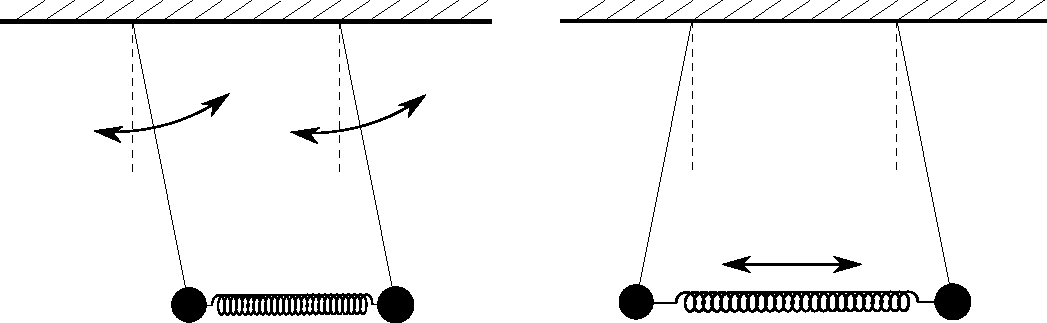
\includegraphics[width=0.7\textwidth]{figures/figure_5.pdf}
        \end{figure}
    \section{Two coupled oscillators}
        Let $x_1$ and $x_2$ denote the distance of the two blocks from $A$. The kinetic and potential energy of the system is then
        \begin{equation*}
            T = \frac{1}{2}m(\dot x_1^2 + \dot x_2^2), \quad V = \frac{1}{2} k (x_1^2 + (x_1 - x_2)^2).
        \end{equation*}
        Writing out the lagrangian in matrix form gives
        \begin{equation*}
            L = \frac{1}{2}m(\dot x_1^2 + \dot x_2^2) + \frac{1}{2}k (2  x_1^2 - 2 x_1  x_2 + x_2^2) = \frac{1}{2}\left(m_{ij}\dot x_i \dot x_j + A_{ij} x_i x_j\right),
        \end{equation*}
        where
        \begin{equation*}
            \bar {\bar m} = m
            \begin{pmatrix}
                1 & 0 \\
                0 & 1 
            \end{pmatrix}
            \quad \bar {\bar A} = k
            \begin{pmatrix*}
                2 & -1 \\
                -1 & 1
            \end{pmatrix*}
        \end{equation*}
        If we introduce $\omega_0^2 = k/m$. This means the equation for the eigenfrequencies is
        \begin{align*} & \det(A - \omega^2m) = 
            \begin{vmatrix}
                2\omega_0^2 - \omega^2& -\omega_0^2 \\
                -\omega_0^2 & \omega_0^2 - \omega^2
            \end{vmatrix}
            = (2\omega_0^2 - \omega^2)(\omega_0^2 - \omega^2) - \omega_0^4 = 2\omega_0^4 - 3 \omega_0^2\omega^2 + \omega^4 - \omega_0^4 \\
            & = (\omega^2)^2 - 3\omega_0^2(\omega^2) + \omega_0^4 =0 \implies \omega^2 = \frac{1}{2} \left(3\omega_0^2 \pm \sqrt{(3\omega_0^2)^2 - 4\omega_0^4}\right) = \frac{3 \pm \sqrt{5}}{2}\omega_0^2.
        \end{align*}
        The equations for the normal coordinates are
        \begin{equation*}
            \begin{dcases*}
                a_{11} = \left(1 - \frac{3 - \sqrt{5}}{2}\right)a_{21} =-\left(\frac{1 + \sqrt{5}}{2}\right)a_{21}\\
                a_{12} = \left(1 - \frac{3 + \sqrt{5}}{2}\right)a_{22} = -\left(\frac{1+\sqrt5}{1+\sqrt 5}\right)\left(\frac{1 - \sqrt{5}}{2}\right)a_{22} = \left(\frac{2}{1 + \sqrt 5}\right) a_{22}.
            \end{dcases*}
        \end{equation*}
        The golden ratio! Here, we picked out one of two possible equations. But as they are linearly dependent (we have inserted $\omega^2$ such that the determinant is zero), we could have chosen either one. In vector form, 
        \begin{equation*}
            \mathbf{a}_1= C_1
            \begin{pmatrix*}
                -1 \\
                \frac{2}{1 + \sqrt 5}
            \end{pmatrix*}
            \quad
            \mathbf{a}_2= C_2
            \begin{pmatrix*}
                \frac{2}{1 + \sqrt 5} \\
                1
            \end{pmatrix*}
        \end{equation*}
        These modes corresponds to vibration in the same and opposite direction. However, this system is not as symmetrical as the last one, so the amplitudes of the oscillations have different absolute values. 

    \section{Oscillating body with two attached pendula}
        The potential energy of the block is $2\frac{1}{2}k x^2$, and using the same small oscillation approximation as in the first exercise the potential energy of both pendula is $\frac{1}{2}mg\ell \theta$. The total potential energy of the system is thus
        \begin{equation*}
            V = kx^2 + \frac{1}{2}\ell(\theta_1^2 + \theta_2^2) = \frac{1}{2} \sum_{ij} A_{ij} q_i q_j, 
        \end{equation*}
        where $(q_1, q_2, q_3) = (x, \theta_1, \theta_2)$ and
        \begin{equation*}
            \bar {\bar A} =
            \begin{pmatrix*}
                2k & 0 & 0 \\
                0 & mgl & 0 \\
                0 & 0 & mgl \\
            \end{pmatrix*}
        \end{equation*}
        When we find the kinetic energy, we must remember that the velocities of the pendula are not only due to the change in $\theta$, but also dependent on how the box moves. The kinetic energy is
        \begin{align*}
            T &= \frac{1}{2} M \dot x^2 + \frac{1}{2}m (\dot x + \ell \dot \theta_1)^2 + \frac{1}{2}m (\dot x + \ell \dot \theta_2)^2\\
            &= \frac{1}{2} (M + 2m) \dot x^2 + \frac{1}{2} m \ell \dot x \theta_1 + \frac{1}{2} m \ell \dot x \theta_2 + \frac{1}{2}m\ell^2\dot \theta_1 + \frac{1}{2}m\ell^2\dot \theta_2 = \frac{1}{2}\sum_{ij}m_{ij}q_iq_j
        \end{align*}
        in matrix form, 
        \begin{equation*}
            \bar {\bar m} = 
            \begin{pmatrix*}
                M + 2m & m\ell & m \ell \\
                m\ell & m\ell^2 & 0 \\
                m\ell & 0 & m\ell^2
            \end{pmatrix*}
        \end{equation*}
        The equation for the eigenfrequencies are 
        \begin{align*} 
            & \det(\bar {\bar A} - \omega^2\bar {\bar m}) = 
            \begin{vmatrix}
                2k - \omega^2(M + 2m) & -\omega^2m\ell & - \omega^2m \ell \\
                -\omega^2m\ell & mg\ell - \omega^2m\ell^2 & 0 \\
                -\omega^2m\ell & 0 & mg\ell - \omega^2m\ell^2
            \end{vmatrix}
            \\
            & = (mg\ell - \omega^2m\ell^2) \Big[(mg\ell - \omega^2m\ell^2)(2k + \omega^2(M + 2m)) - (\omega^2m \ell)^2\Big] 
            - (\omega^2m\ell)^2 \left(mg\ell - \omega^2m\ell^2\right) \\ 
            & = (mg\ell - \omega^2m\ell^2) \bigg(2mg\ell k  - \omega^2[2m\ell^2k - (M + 2m)mg\ell] + \omega^4Mm\ell^2 \bigg) = 0.
        \end{align*}
        Thus, either $\omega^2 = \omega_1^2 = g/\ell$, or (after dividing by $Mm\ell^2$)
        \begin{align*}
            & \omega^4 - \left(\frac{2k}{M} + \frac{g}{\ell}\left[1 + 2 \frac{m}{M}\right]\right) \omega^2 + 2\left(\frac{gk}{\ell M}\right) = 0\\
            \implies  &\omega^2 = \frac{k}{M} + \frac{1}{2}\frac{g}{\ell}\left[1 + 2 \frac{m}{M}\right]\pm \sqrt{\left(\frac{k}{M} + \frac{1}{2}\frac{g}{\ell}\left[1 + 2 \frac{m}{M}\right]\right)^2 - 2 \frac{gk}{\ell M}}.
        \end{align*}

    \section{Double pendulum}
        We have found the kinetic and potential energy of the double pendulum before,
        \begin{equation*}
            T = m\ell^2\dot \theta_1^2 + m \ell^2 \cos(\theta_1 - \theta_2)\dot \theta_1^2 \dot \theta_2^2 + \frac{1}{2}m \ell^2 \dot \theta_2^2, \quad
            V = -mg\ell \cos(\theta_1) - mg \ell \cos(\theta_2).
        \end{equation*}
        With the small angle approximation this becomes
        \begin{equation*}
            T = \frac{1}{2}m\ell^2\left(2\dot \theta_1^2 + 2\dot \theta_1 \dot \theta_2 + \dot \theta^2_2 \right), \quad
            V = \frac{1}{2}mg \ell \left(2\theta_1^2 + \theta_2^2\right) + \mathrm{const.}
        \end{equation*}
        In matrix form, 
        \begin{equation*}
            \bar {\bar m} = 
            \begin{pmatrix*}
                2m \ell^2 & m \ell^2 \\
                m \ell^2 & m \ell^2
            \end{pmatrix*}
            \quad
            \bar {\bar A} = 
            \begin{pmatrix*}
                2mg\ell & 0 \\
                0 & mg\ell
            \end{pmatrix*}
        \end{equation*}
        Defining $\omega_0 = \sqrt{g/\ell}$, the eigenfrequencies are given by
        \begin{align*}
            & \det(\bar {\bar A} - \omega^2 \bar {\bar m}) = m \ell
            \begin{pmatrix*}
                2(\omega_0^2 -\omega^2 ) & -\omega^2 \\
                -\omega^2 & \omega_0^2 - \omega^2
            \end{pmatrix*}
            = (2[\omega^2 - \omega_0^2]^2 - \omega^4) = 0 \\
            \implies & \omega^4 - 4 \omega_0^2 \omega^2 + 2\omega_0^4 = 0 \implies \omega^2 = 2\omega^2 \pm \sqrt{4\omega_0^4 - 2\omega_0^2} = \left(2 \pm \sqrt 2\right) \omega_0^2.
        \end{align*}
        The eigenvectors are (choosing the equation from the lower row)
        \begin{equation*}
            (-1 \mp \sqrt 2) a_{1i} - (2 \pm \sqrt 2)a_{2i} = 0 \implies a_{1i} = -\frac{1 \pm \sqrt 2}{2 \pm \sqrt 2} a_{2i} =  -\frac{1}{\sqrt 2}\frac{1 \pm \sqrt 2}{\sqrt 2 \pm 1} a_{2i} = \mp \frac{1}{\sqrt 2} a_{2i}
        \end{equation*}
        In vector form, they are
        \begin{equation*}
            \mathbf{a}_1 = c_1
            \begin{pmatrix*}
                1 \\
                - \sqrt{2}
            \end{pmatrix*}
            , \quad \mathbf{a}_2 = c_2
            \begin{pmatrix*}
                1 \\
                \sqrt 2
            \end{pmatrix*}
        \end{equation*}
\end{document}
